\documentclass[10pt,landscape]{article}
\usepackage{graphicx}
\usepackage{amssymb,amsmath,amsthm,amsfonts}
\usepackage{multicol,multirow}
\usepackage{calc}
\usepackage{ifthen}
\usepackage[landscape]{geometry}
\usepackage[colorlinks=true,citecolor=blue,linkcolor=blue]{hyperref}


\ifthenelse{\lengthtest { \paperwidth = 11in}}
    { \geometry{top=.5in,left=.5in,right=.5in,bottom=.5in} }
	{\ifthenelse{ \lengthtest{ \paperwidth = 297mm}}
		{\geometry{top=1cm,left=1cm,right=1cm,bottom=1cm} }
		{\geometry{top=1cm,left=1cm,right=1cm,bottom=1cm} }
	}
\pagestyle{empty}
\makeatletter
\renewcommand{\section}{\@startsection{section}{1}{0mm}%
                                {-1ex plus -.5ex minus -.2ex}%
                                {0.5ex plus .2ex}%x
                                {\normalfont\large\bfseries}}
\renewcommand{\subsection}{\@startsection{subsection}{2}{0mm}%
                                {-1explus -.5ex minus -.2ex}%
                                {0.5ex plus .2ex}%
                                {\normalfont\normalsize\bfseries}}
\renewcommand{\subsubsection}{\@startsection{subsubsection}{3}{0mm}%
                                {-1ex plus -.5ex minus -.2ex}%
                                {1ex plus .2ex}%
                                {\normalfont\small\bfseries}}
\makeatother
\setcounter{secnumdepth}{0}
\setlength{\parindent}{0pt}
\setlength{\parskip}{0pt plus 0.5ex}
% -----------------------------------------------------------------------

\title{Coffee Oreo Cheesecake}

\begin{document}

\raggedright
\footnotesize

\begin{center}
     \Large{\textbf{Carrot Cake}} \\
     \small{\today}
\end{center}
\begin{multicols}{3}


\section{Notes}
\begin{tabular}{l l} 
 Yields & 12 servings \\ 
 Prep Time & 1 hour \\ 
 Chill Time & 12 hours \\ 
 Cook Time & 65 minutes \\
 Bake Temperature & 325\textdegree F \\
 Utensil Type & Metal
\end{tabular}

\bigskip

\section{Ingredients}
\begin{tabular}{l l} 
 Cream Cheese & 24 oz \\ 
 Coffee & 1/3 cup \\
 White Sugar & 180g \\
 Whole Eggs & 4 \\
 Oreo Crumbs& 2 cups \\ 
 Butter & 4 tbsp  \\
\end{tabular}

\vfill\null
\columnbreak

\section{Instructions}
\begin{enumerate}
    \item In a 9 inch pan, make an Oreo crust with Oreo crumbs and butter
    \item In a separate container, Whisk cream cheese until smooth
    \item While whisking, add coffee in batches of 3
    \item While whisking, add sugar in batches of 3
    \item While whisking, add one egg at a time until egg yolk is dissolved
    \item DO NOT over beat mixture
    \item Pour the batter to the pan and bake for 65 - 70 minutes at 325 in a water bath\textdegree F
    \item Ideally, the center should be jiggly while the sides should have firmed up. 
    \item Turn off the oven and leave the oven door ajar until cheesecake cools down completely.
    \item Place the cheesecake in the fridge for 12 hrs.
    
\end{enumerate}
\bigskip
CAUTION: All ingredients must be room temperature
\vfill\null
\columnbreak
 
\section{Results}
\begin{itemize}
    \item Cheesecake came out well. The ore's and coffee flavor contrast each other pretty well. 

\end{itemize}
\bigskip
\section{Try out next batch}
\begin{itemize}
    \item Make a stiffer Oreo crumb base
    \item Wait for cheesecake to completely cool down before placing it in the fridge. 
\end{itemize}
\vfill\null
\columnbreak
\end{multicols}

\section{Images}
\newcommand{\widthsize}{15cm}
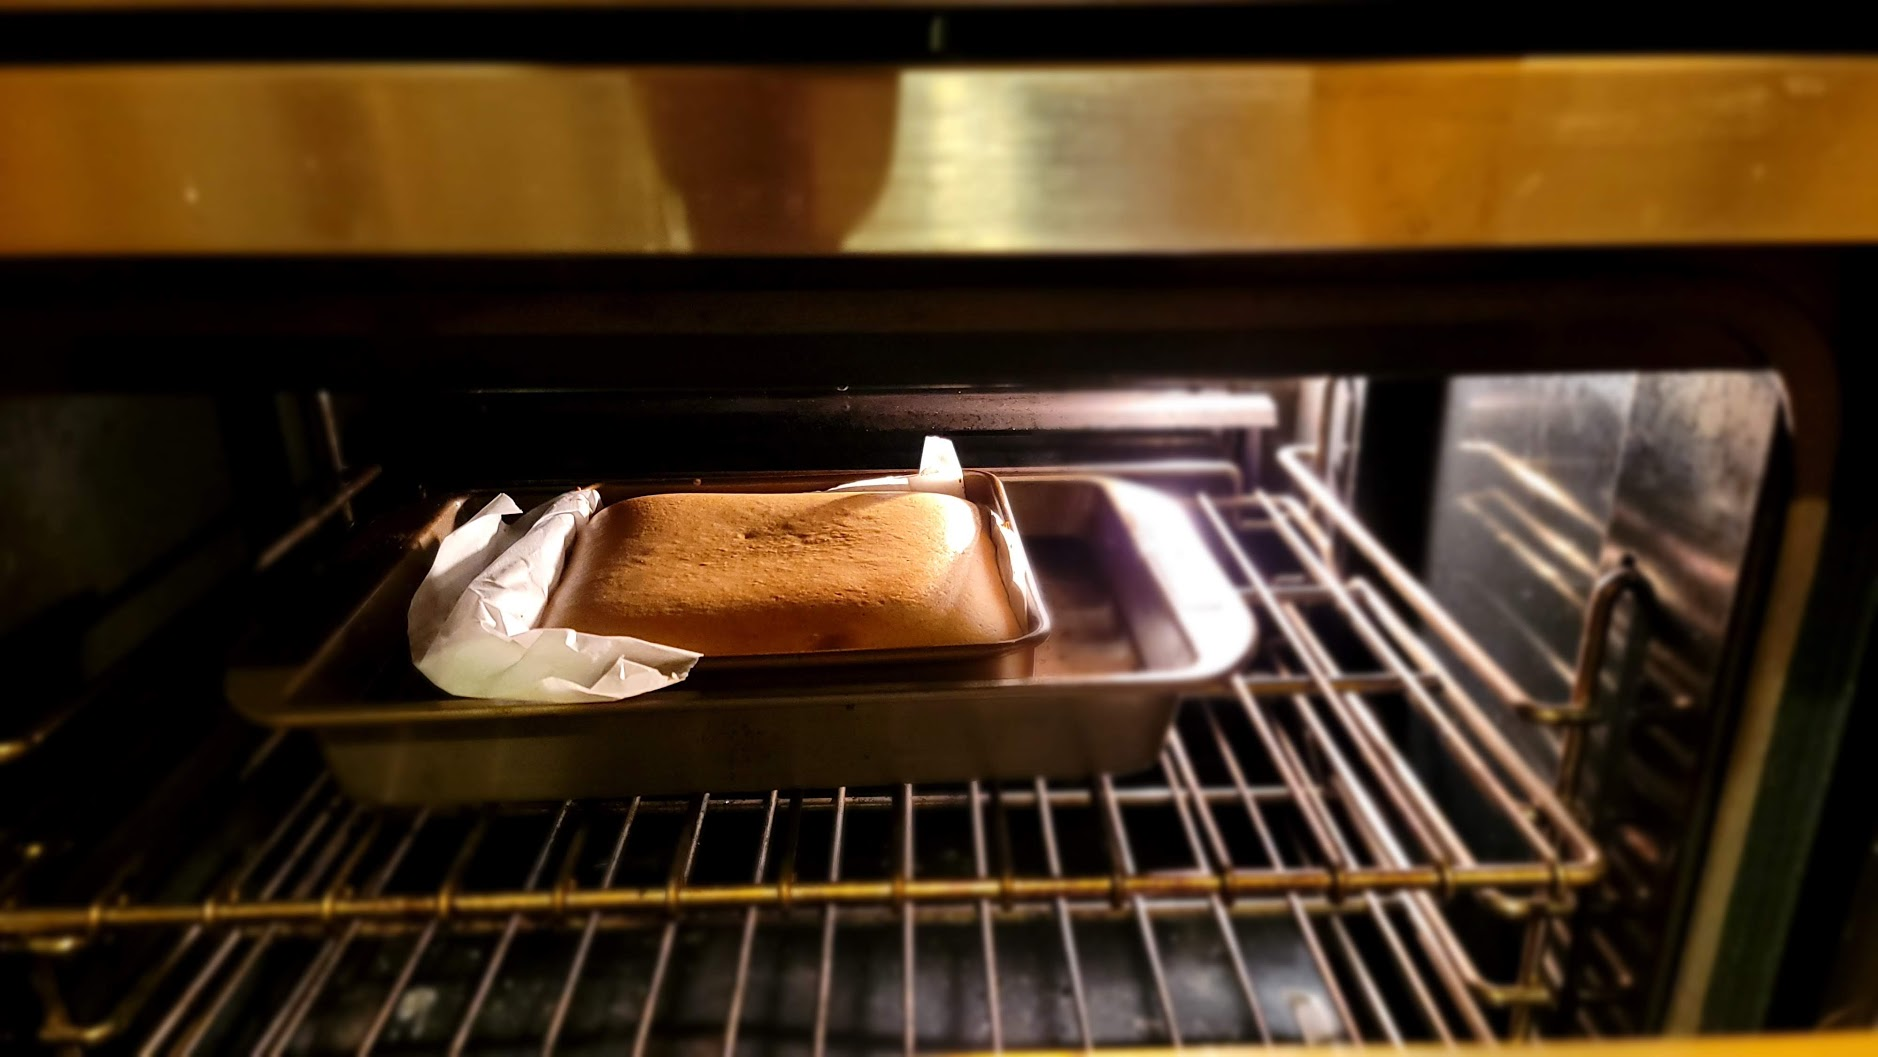
\includegraphics[width=\widthsize]{g1.jpg}


\bigskip
Inspired from thefirstyear's Cheesecake recipe https://www.youtube.com/watch?v=gP3gWS2S5EY
\end{document}
